\section[Background]{Background}

\begin{frame}[fragile]{The Transformer Architecture}

\begin{tabular}{cl}
    \begin{tabular}{c}
        \begin{tabular}{p{0.3\textwidth}p{\textwidth}}
            \scriptsize{
                The Transformer block\footfullcite{DBLP:conf/nips/VaswaniSPUJGKP17}.
            } \\
            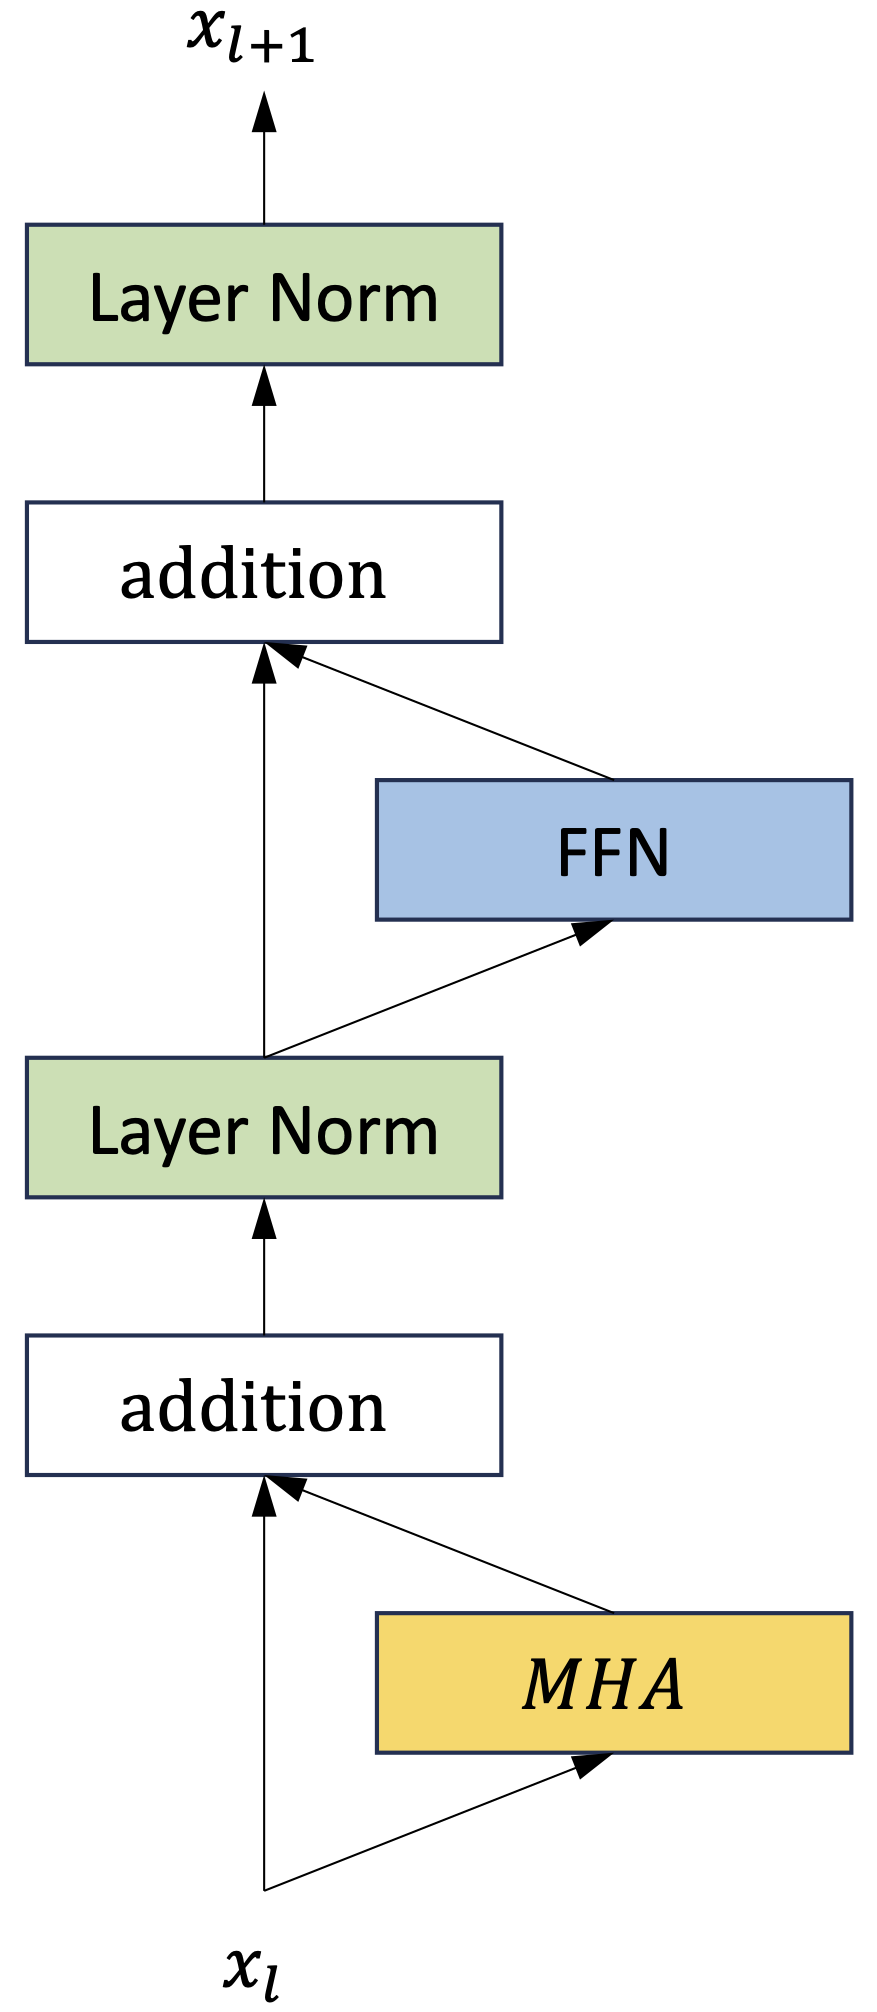
\includegraphics[scale=0.4]{"../Formalize_Flash_Attention/figures/Transformer-block.pdf"}
        \end{tabular}
    \end{tabular} &
    \begin{tabular}{p{13.5cm}l}
        \parbox{0.5 \linewidth}{
            \begin{itemize}
                \item The transformer model consists of $n_{\text{layers}}$ blocks that are stacked on top of each other.
                \item Learnable parameters in a Transformer block:
                \item[] 
                \scriptsize{
                \begin{tabular}{lll}\hline
                    \textbf{Components}& \textbf{Parameters} & \textbf{Shape} \\ \toprule[1.5pt]
                    MHA & $W_Q^i$,$W_K^i$,$W_V^i$,$W_O^i$ & $[d, d]$ \\
                    MHA & $b_Q^i$,$b_K^i$,$b_V^i$,$b_O^i$ & $[1, d]$ \\
                    layer norm & $\gamma$, $\beta$ & $[1, d]$ \\
                    FFN & $W_1^i$ & $[d, 4d]$ \\
                    FFN & $b_1^i$ & $[1, 4d]$ \\
                    FFN & $W_2^i$ & $[4d, d]$ \\
                    FFN & $b_2^i$ & $[1, d]$ \\ \hline
                    \text{In Total}&& \textcolor{red}{$12d^2+13d$}\\\hline
                \end{tabular}
                }
            \end{itemize}
        }
    \end{tabular}
\end{tabular}
\end{frame}

\begin{frame}{Estimating Storage Requirements for LLM Weights}
    \textbf{LLMs are too large to fit in the memory of a single GPU device.} Inference performance for large Transformer models can be limited by memory capacity.
    
    \begin{itemize}
        \item Storage required for LLM weights:
        \item[]
        \scriptsize{
            \begin{tabular}{lcccccc}
            \textbf{Model} & $\#\textbf{parameters}$\footnote{$\#\textbf{paramters}$ = $n_{\text{layers}}*(12d^2+13d)$. The parameters are counted in a manner that excludes word embedding and the last softmax parameters used to predict the following word.} & $n_{\text{layers}}$ & $d$ & $n_{\text{heads}}$ & $d_{\text{head}}$& $\#\textbf{storage}(GB)$\footnote{$\#\textbf{storage}$ is counted for single precision floating point number = $\#\textbf{parameters}$ * 4 / 1024 / 1024 / 1024 }\\\toprule[1.5pt]
            $\text{BERT}_{\text{base}}$ &84.94 M&12 &768 &12&64&0.3164\\
            $\text{BERT}_{\text{large}}$ &302.00 M&24 &1024 &16&64&1.1250\\
            GPT-3 small &84.94 M&12&768&12&64&0.3164\\
            GPT-3 medium &302.00 M&24&1024&16&64&1.1250 \\
            GPT-3 large &679.50 M&24&1536&16&96&2.5313\\
            GPT-3 13B &12.68 B&40&5140&40&128&47.2421 \\
            GPT-3 175B &173.95 B&96&12288&96&128&648.0006\\
        \end{tabular}
        }
        \normalsize{
        \item Other storage: Activations, \hl{K-V cache}!
        }
    \end{itemize}
    \end{frame}

\begin{frame}{LLM inference}
\footnotesize{
    \begin{itemize}
        \item[] \center{\hl{Prefill Stage}: prompts processing has large parallelism}
            \begin{enumerate}
                \item cache K-V for prompts
                    \begin{align*}
                        \mathbf{x}_K^i &= \mathbf{x}^i \cdot W_{K}^i \\
                        \mathbf{x}_V^i &= \mathbf{x}^i \cdot W_{V}^i
                    \end{align*}
                \item predict next token
                \begin{align*}
                    \mathbf{x}_Q^i &= \mathbf{x}^i \cdot W_{Q}^i \\
                    \mathbf{x}_O^i &= \textcolor{red}{\text{layernorm}}\left(\textcolor{red}{\text{softmax}}\left(\frac{\mathbf{x}_Q^i(\mathbf{x}_K^i)^T}{\sqrt{d}}\right) \mathbf{x}_V^i W_O^i + \mathbf{x}^i\right) \\
                    \mathbf{x}^{i+1} &= \textcolor{red}{\text{layernorm}}\left(\text{relu}\left(\mathbf{x}^i_OW_1^i\right)W_2^1+\mathbf{x}_O^i\right)
                \end{align*}
            \end{enumerate}
        \item[] \center{\hl{Decode Stage}: next token generation has insufficient parallelism}
            \begin{enumerate}
                \item update K-V for prompts
                        \begin{align*}
                            \mathbf{x}_K^i&\leftarrow\textcolor{red}{\text{concat}}({\mathbf{x}_K^i}, \mathbf{t}^i\cdot W_K^i) \\
                            \mathbf{x}_V^i&\leftarrow\textcolor{red}{\text{concat}}({\mathbf{x}_V^i}, \mathbf{t}^i\cdot W_V^i) 
                        \end{align*}
                \item predict next token, the same as above, but each time a token
            \end{enumerate}
    \end{itemize}
}
\end{frame}

\begin{frame}{Two stages in LLM inference}
    \begin{figure}
        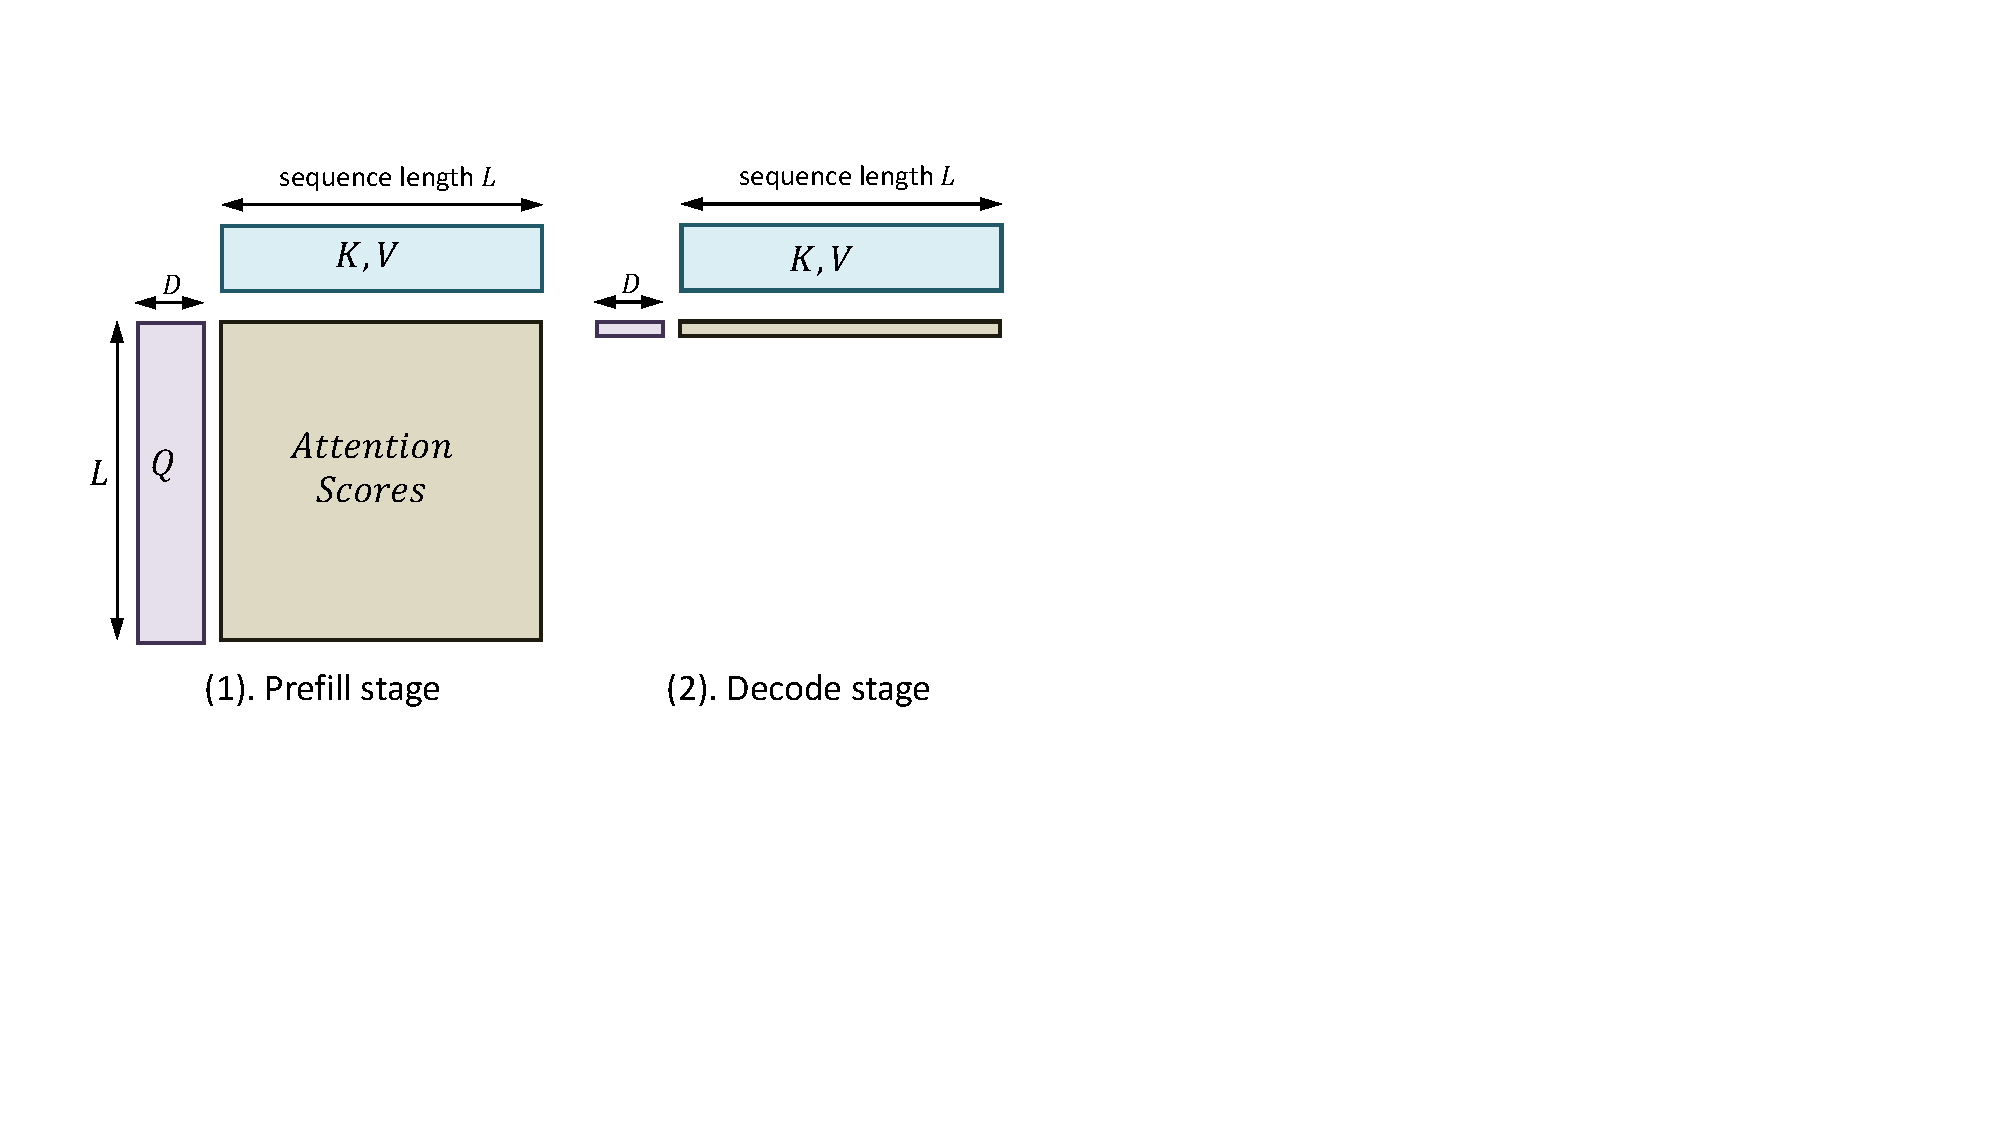
\includegraphics[width=0.7\linewidth]{./images/two-stages-in-llm-inference.pdf}
        \caption{There is a significant change in batch size between the two stages of LLM inference.}
    \end{figure}
\end{frame}

\begin{frame}{Performance Breakdown of a Transformer Block}
    \begin{figure}
        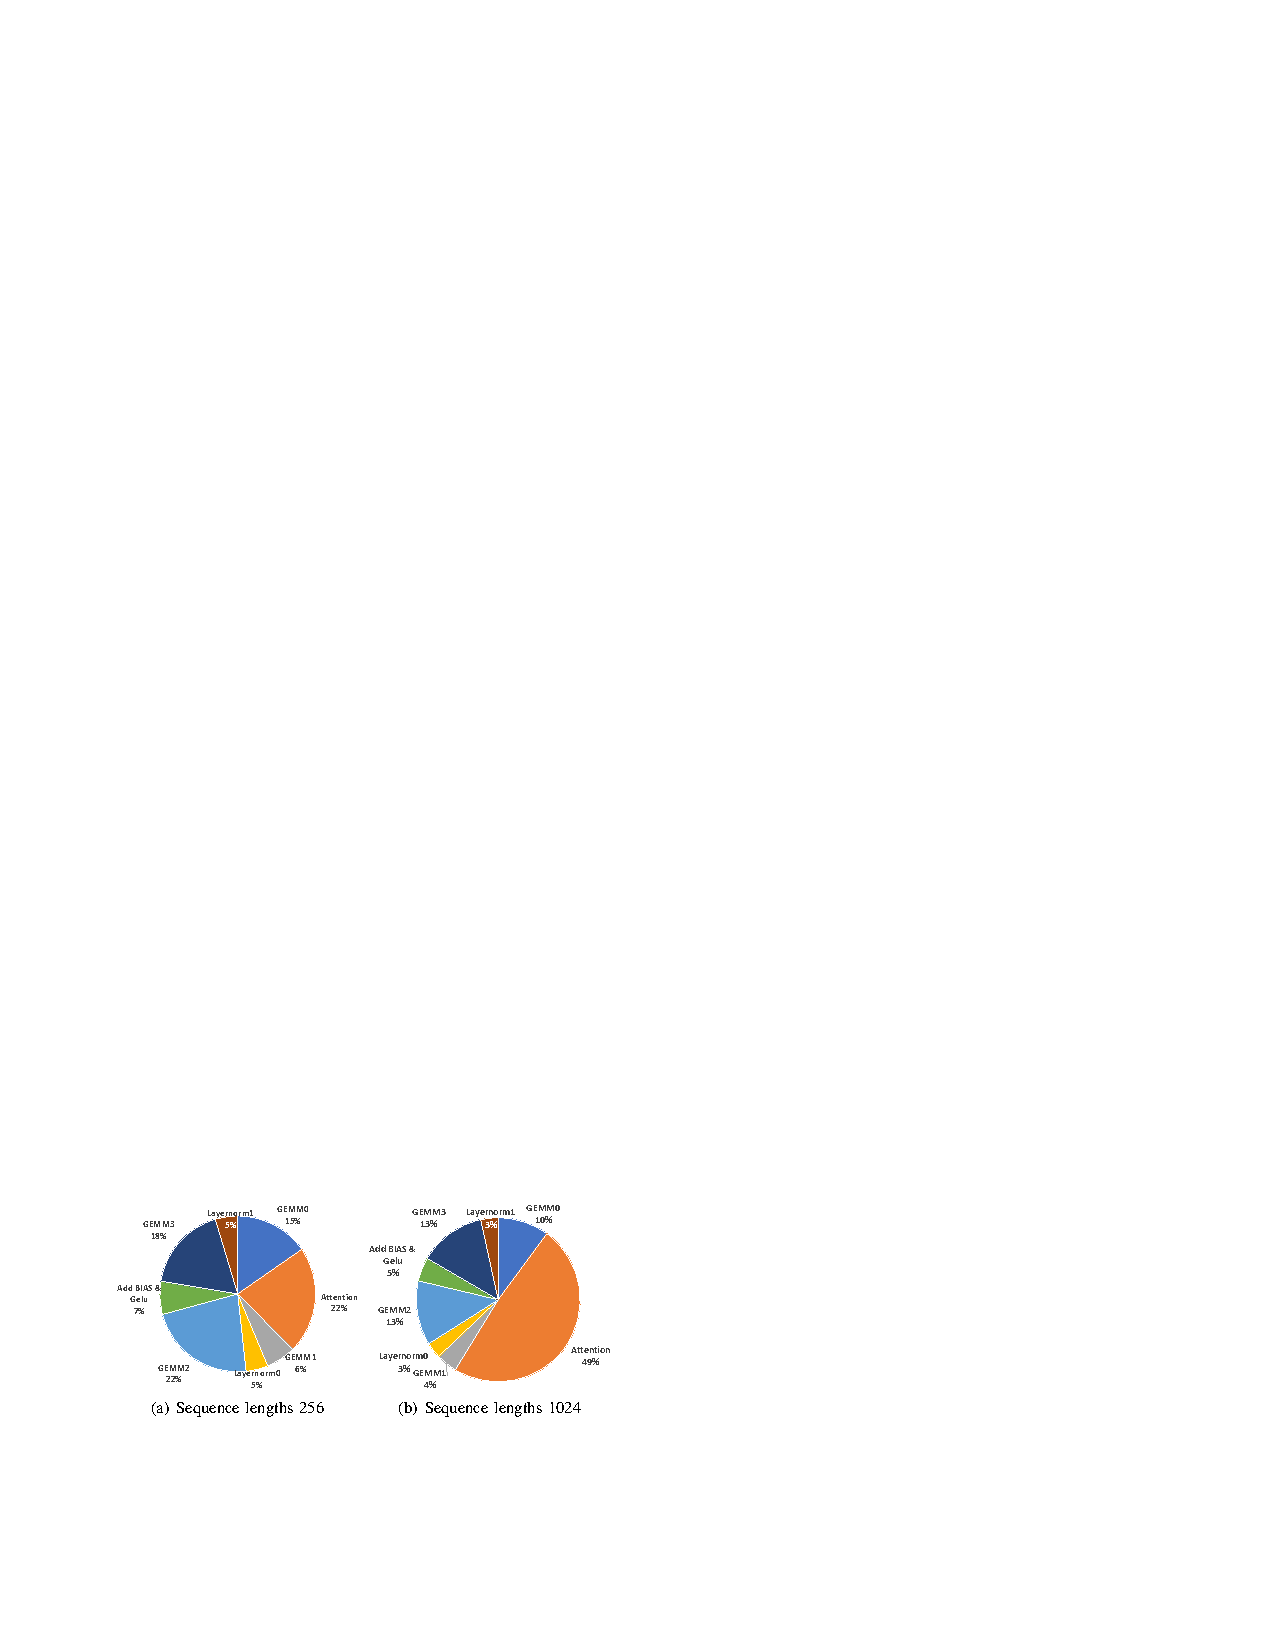
\includegraphics[width=0.7\linewidth]{./images/BERT-performance-breakdown.pdf}
        \caption{A performance breakdown of a single Transformer block\footfullcite{DBLP:journals/corr/abs-2210-03052}.}
    \end{figure}

    \footnotesize{
    \begin{enumerate}
        \item Transformer block is memory bounded.
        \item The computational complexity of MHA is quadratic to sequence length.
    \end{enumerate}
    }
\end{frame}

\begin{frame}[fragile]{Distinction Between Transformer Training and Inference:}

\textbf{Small batch size}.

\begin{enumerate}
\item Kernels are not well optimized for small batch size.

The use of \hl{skinny matrix multiplication} is a result of having a small batch size, where the batch size $N$ is much smaller than the dimensionality $d$.
\begin{align*}
 \mathbf{x}_Q^i &= \mathbf{x}^{i}W_{Q}^i & [N, d] &= [N,d] \times [d, d]\\
 \mathbf{y}_1^i &= \mathbf{x}_O^{i}W_1^i & [N, 4d] &= [N,d] \times [d, 4d]\\
 \mathbf{y}_2^i &= \mathbf{y}_1^{i}W_2^i & [N, d] &= [N,4d] \times [4d, d]\\
\end{align*}
\item \hl{Insufficient of parallelism} and performance is limited by memory bandwidth in reading weights.

\end{enumerate}
\end{frame}

\begin{frame}{FlexGen, ByteTransformer, and DeepSpeed Inference}
    \scriptsize{
        \begin{tabular}{lccc}
            &\textbf{FlexGen}\footfullcite{DBLP:journals/corr/abs-2303-06865}& \textbf{ByteTransformer\footfullcite{DBLP:journals/corr/abs-2210-03052}} & \textbf{\makecell{DeepSpeed \\Inference\footfullcite{DBLP:conf/sc/AminabadiRALLZRSZRH22}}} \\ \toprule[1.5pt]
            Throughput-oriented& yes & no & no\\
            Latency-oriented& no & yes & yes\\
            SLA& not discussed & not discussed & not discussed\\\hline
            Model&OPT-175B&BERT-like&\makecell{Dense Transformer\\MoE Transformer}\\
            Optimized Kernels&not discussed &\makecell{\textcolor{red}{yes}\\\textcolor{red}{for variable length}}&\makecell{yes\\\textcolor{red}{for small batch size}}\\
            Kernel Fusion&not discussed&yes&yes\\
            Multi-GPU&\textcolor{red}{yes}&no&\textcolor{red}{yes}\\
        \end{tabular}
    }
\end{frame}